\documentclass[openbib]{article}

\usepackage{color}
\usepackage{float}
\usepackage{ctex}
\usepackage{mathtools}
\usepackage{amsmath}
\usepackage{graphicx}
\usepackage{fontspec}
\graphicspath{{figures/}}
\renewcommand{\contentsname}{\centerline{目录}}

\begin{document}
	
	%	kited
	\title{实验室还原卡部署}
	
%ls 
	
	\maketitle
	
	\newpage
	\tableofcontents
	\newpage
\section{安装还原卡环境}
安装本系统前,请先将硬盘重要数据进行备份,避免造成安装过程导致数据丢失!
\begin{figure}[htbp]
	\centering
	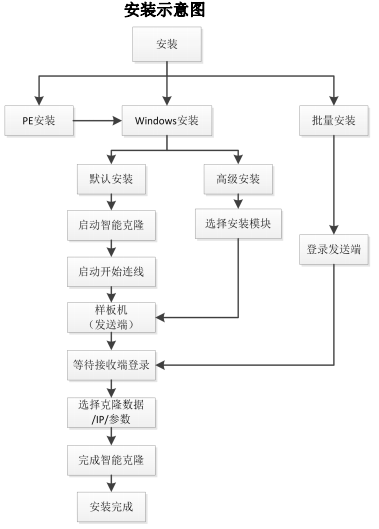
\includegraphics[scale=0.4]{安装示意图}
\end{figure}
\subsection{安装Windows}
1.开机按delte进Bios系统,Boot选项中的Boot mode select 为UEFI,Boot选项中的Boot option \#1选为UEFI USB CD/DVD....
\begin{figure}[htbp]
	\centering
	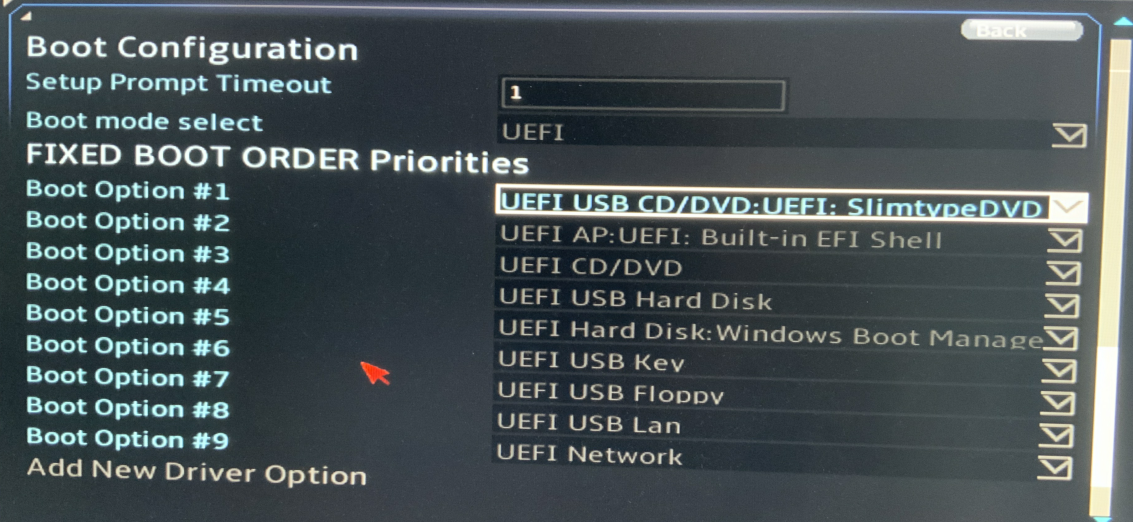
\includegraphics[scale=0.3]{1}
\end{figure}

2.点击Save\&Exit中的Discard changes and Exit 中的Save Changes and Reset。
\begin{figure}[htbp]
	\centering
	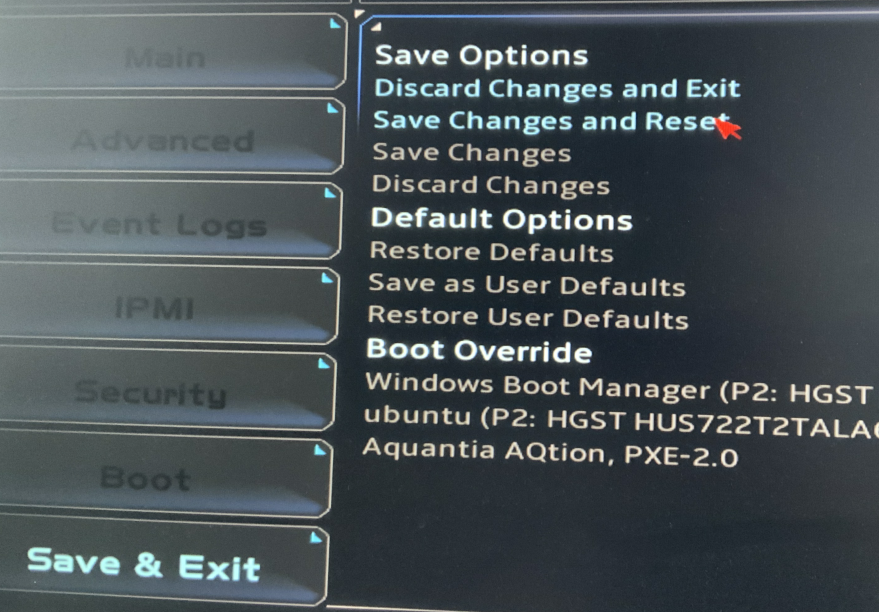
\includegraphics[scale=0.3]{2}
\end{figure}

3.点击ok。
\begin{figure}[htbp]
	\centering
	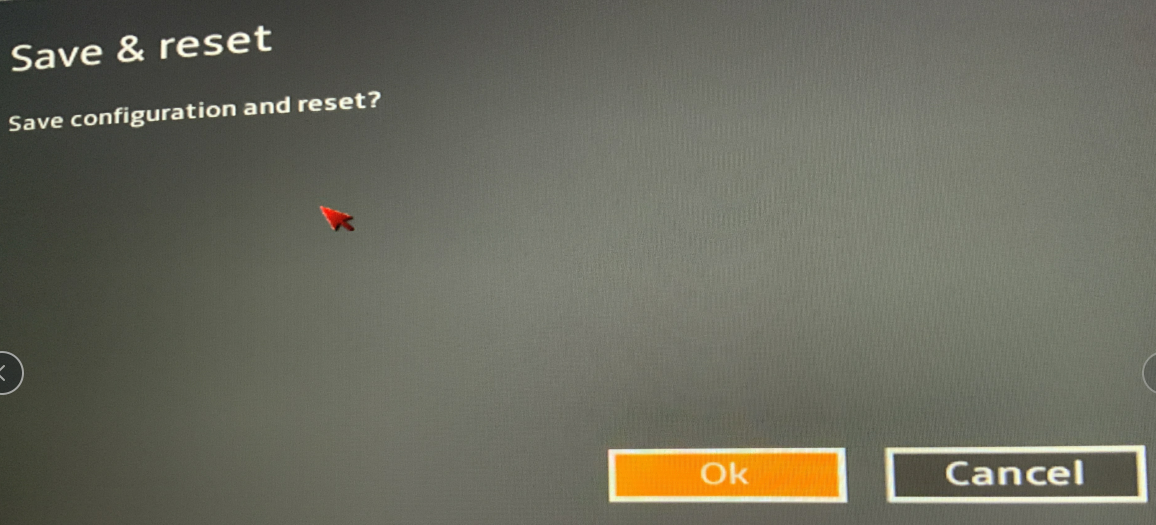
\includegraphics[scale=0.24]{3}
\end{figure}

4.电脑重启,将win10光盘放入移动光驱中,插上USB接口(注意两个都要插)直到出现下图,按任意键继续。
\begin{figure}[htbp]
	\centering
	
\includegraphics[scale=0.3]{4}
\end{figure}

5.出现以下窗口。点击现在安装。
\begin{figure}[H]
	\centering
	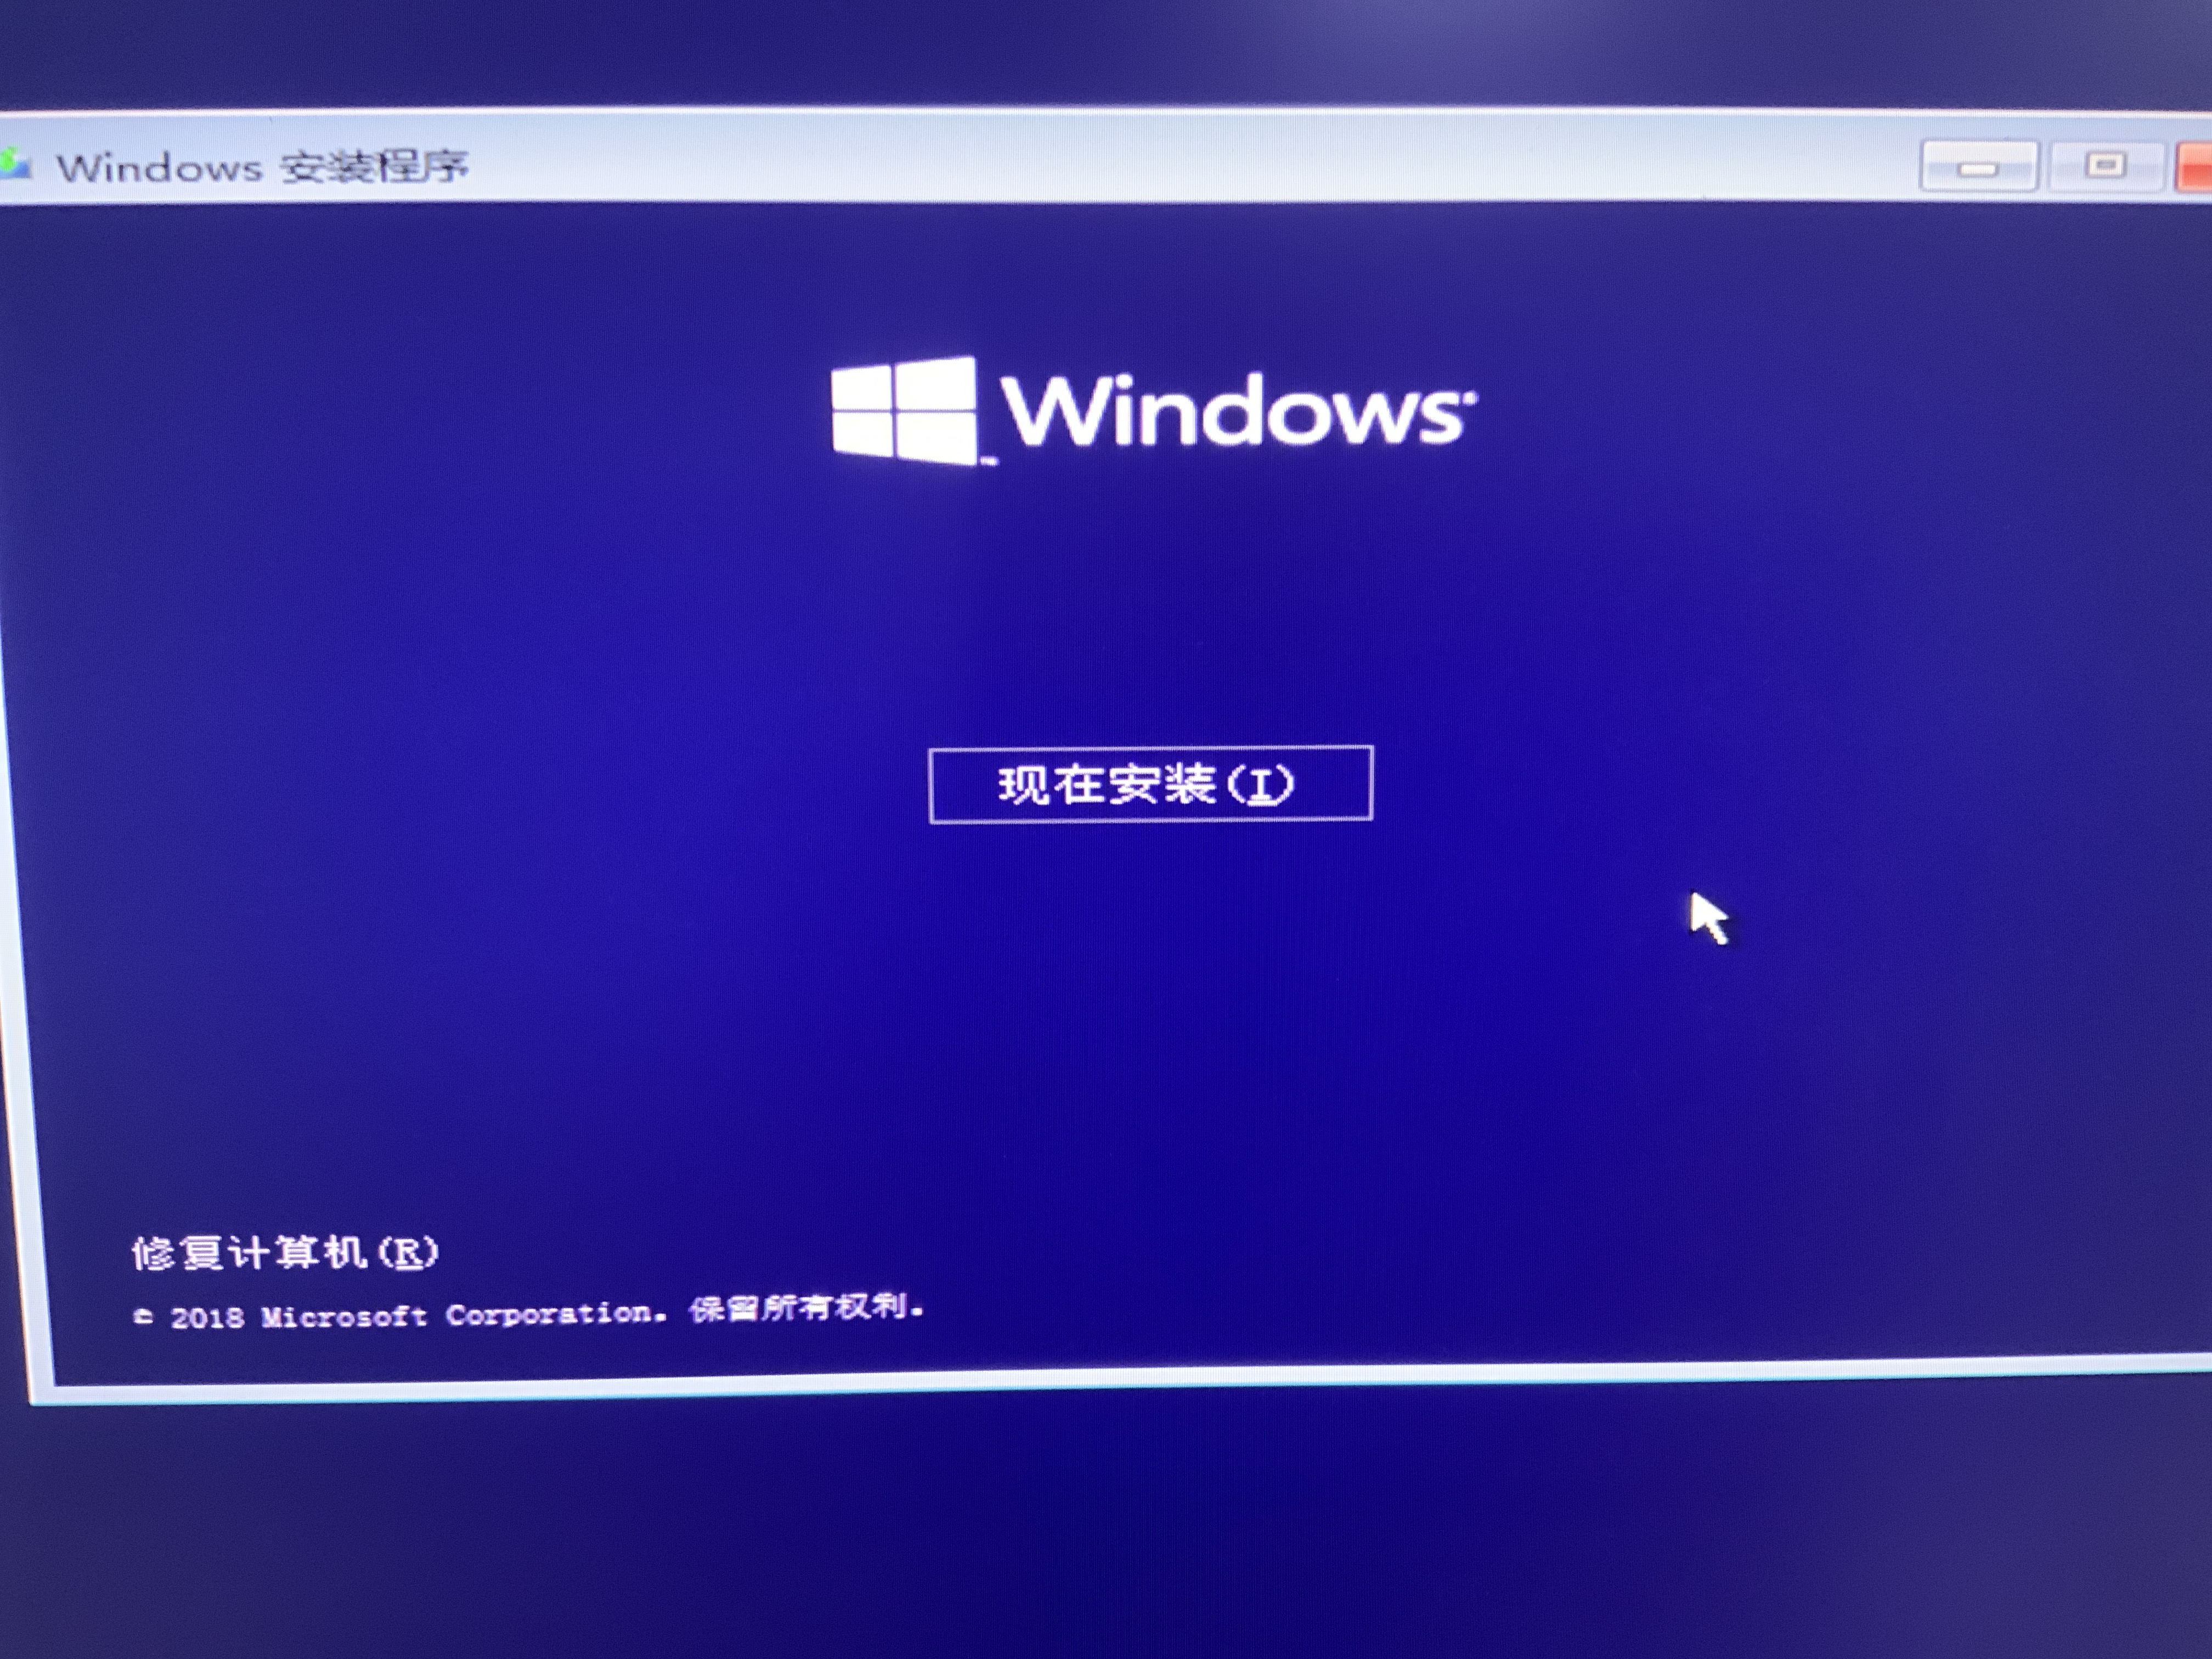
\includegraphics[scale=0.05]{5}
\end{figure}

如果出现以下情况,请拿出磁盘小心擦拭,在放回移动光驱中。重新启动电脑。
\begin{figure}[H]
	\centering
	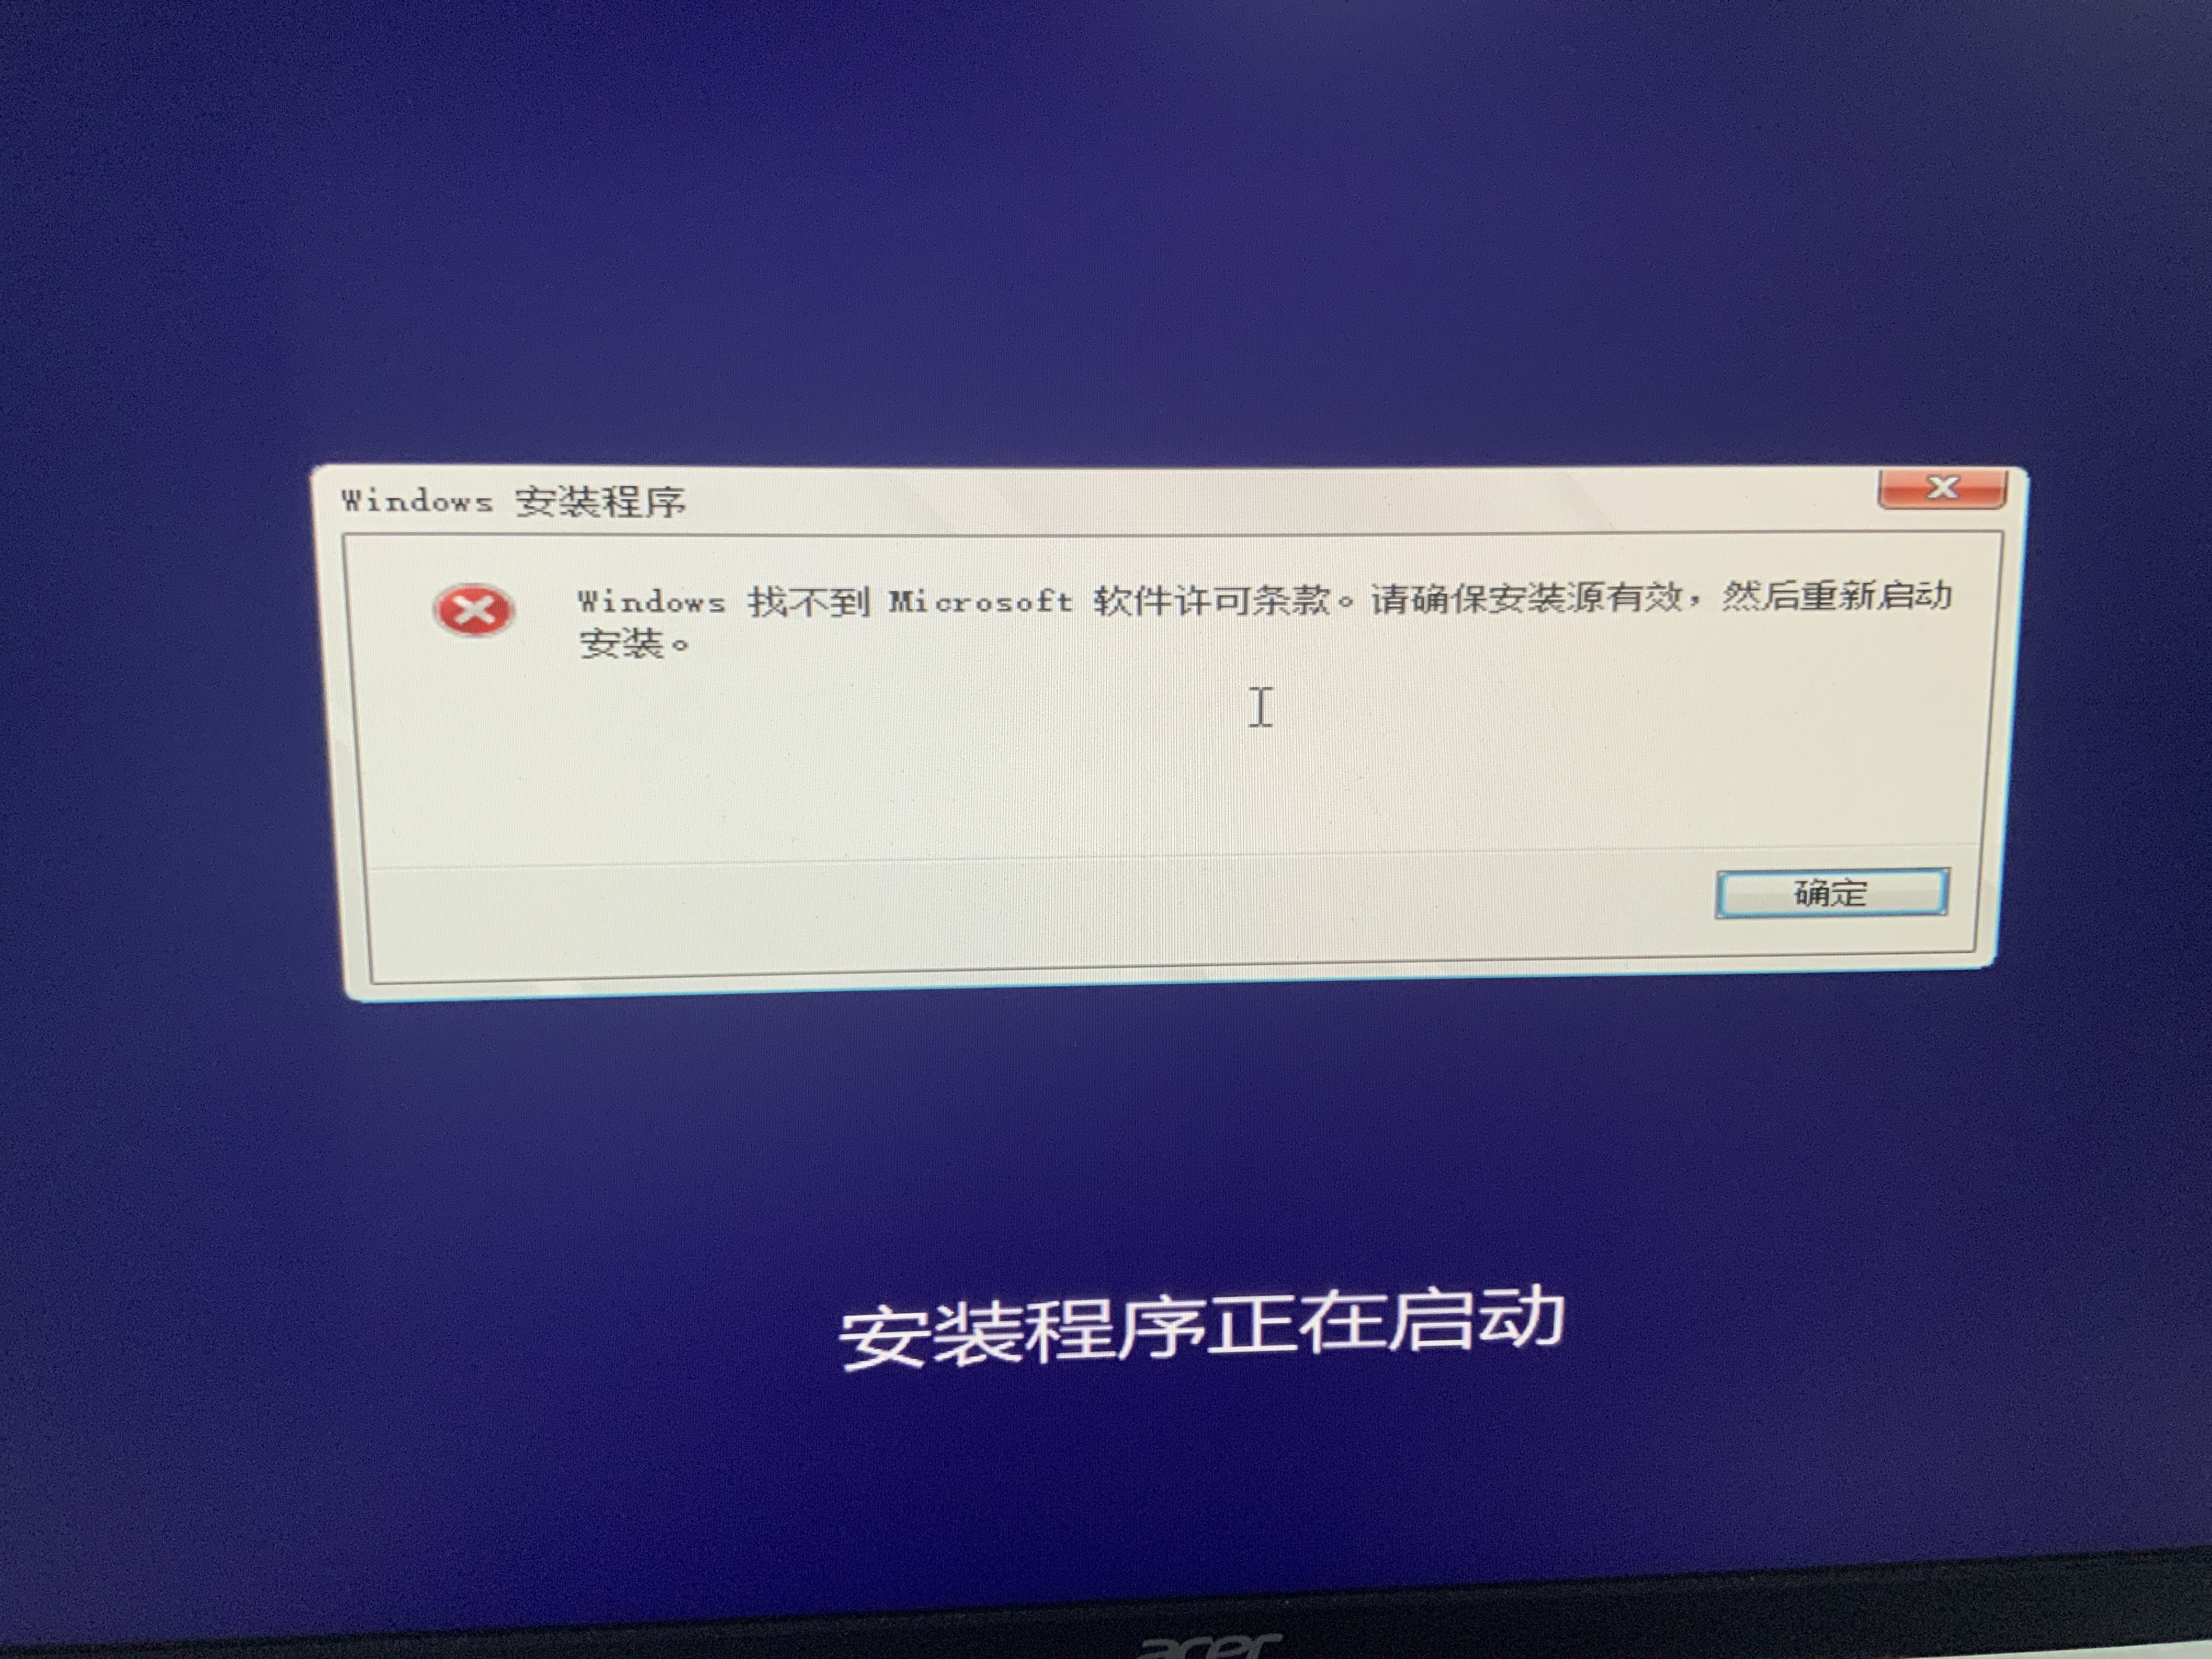
\includegraphics[scale=0.05]{5.1}
\end{figure}

直到出现如图的窗口
\begin{figure}[htbp]
	\centering
	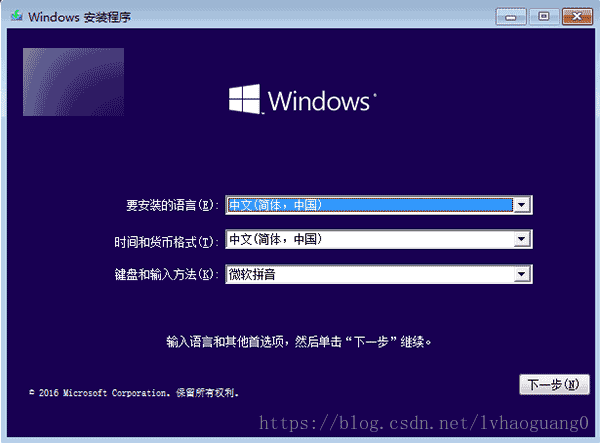
\includegraphics[scale=0.3]{6}
\end{figure}

6.到上图界面后,按下Shift+F10调出命令提示符,如下图。
\begin{figure}[htbp]
	\centering
	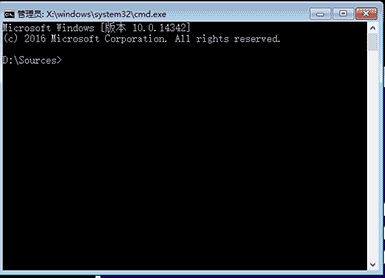
\includegraphics[scale=0.25]{7}
\end{figure}

7.输入diskpart命令后按回车键,进入DISKPART工具,如图所示。
\begin{figure}[htbp]
	\centering
	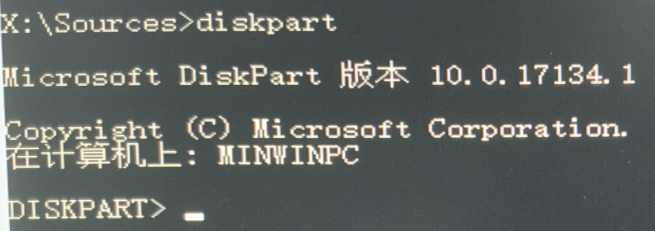
\includegraphics[scale=0.25]{8}
\end{figure}

8.输入list disk命令后按回车键,列出已有的硬盘,如图所示。
\begin{figure}[H]
	\centering
	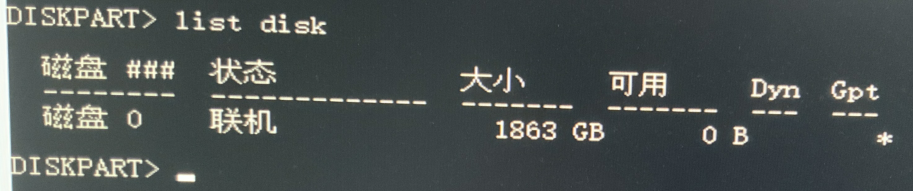
\includegraphics[scale=0.3]{9}
\end{figure}

9.输入select disk 0,选定编号为0的磁盘。(每台电脑情况可能不一样,可将0变为您想安装的盘的编号)
\begin{figure}[htbp]
	\centering
	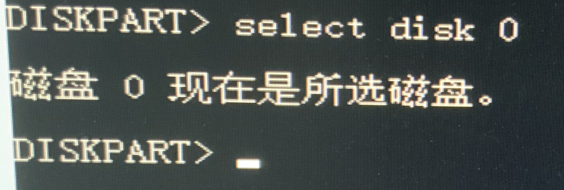
\includegraphics[scale=0.3]{10}
\end{figure}

10.执行clean命令清除该硬盘上的所有分区,此时会清除所有硬盘数据,如下图所示。
\begin{figure}[H]
	\centering
	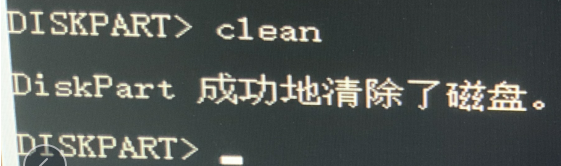
\includegraphics[scale=0.3]{11}
\end{figure}

11.执行convert gpt命令将该硬盘转换成GPT分区表,如下图所示。
\begin{figure}[htbp]
	\centering
	
\includegraphics[scale=0.3]{12}
\end{figure}

12.创建EFI分区,执行create partition efi size=200(分区大小为200MB),如下图所示。
\begin{figure}[H]
	\centering
	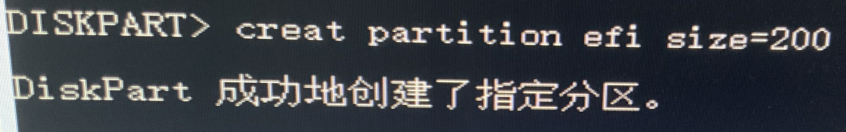
\includegraphics[scale=0.3]{13}
\end{figure}

13.创建MSR分区,执行create partition msr size=200(微软系统保留分区),如下图所示
\begin{figure}[htbp]
	\centering
	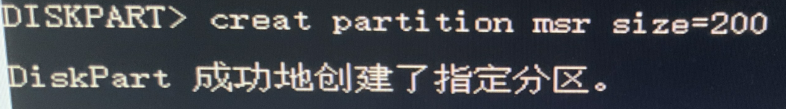
\includegraphics[scale=0.3]{14}
\end{figure}

14.创建主分区,执行create partition primary size=xxx(具体大小根据你的要求而定,作为系统分区来说,命令为create partition primary size=512000,方便系统有足够周转空间)
\begin{figure}[htbp]
	\centering
	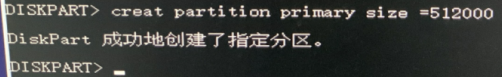
\includegraphics[scale=0.3]{15}
\end{figure}

\textbf{特别说明,设置磁盘大小的代码之间没有空格,即size=xxx之间没空格}

15.关闭窗口,选定语言和键盘等一系列信息后点击下一步,之后点击我接受许可条款,点击下一步。选定自定义安装。
\begin{figure}[H]
	\centering
	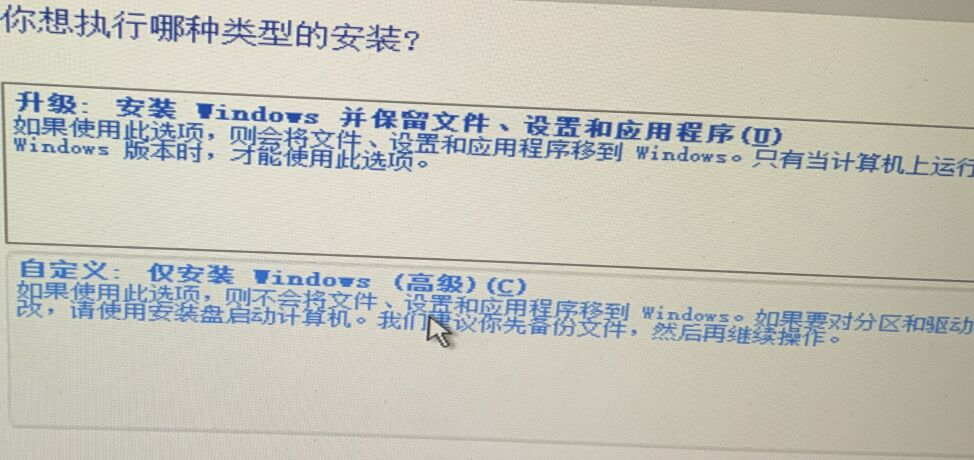
\includegraphics[scale=0.26]{16}
\end{figure}

16.选定您之前分出来的主分区,点击下一步。
\begin{figure}[htbp]
	\centering
	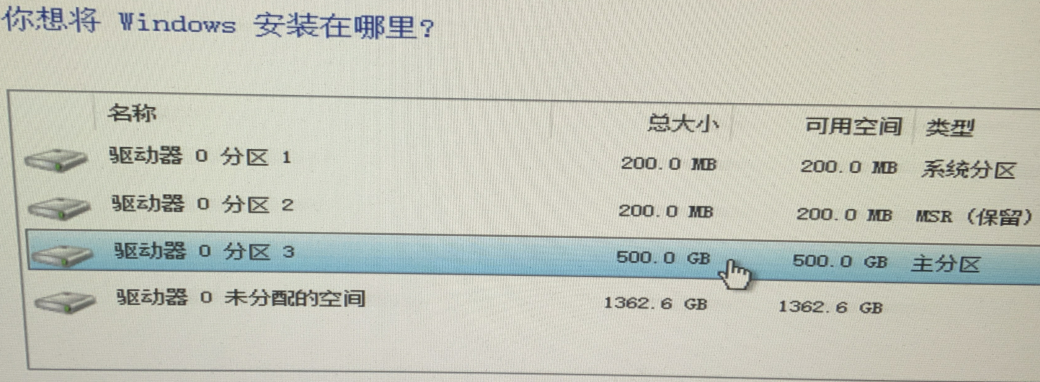
\includegraphics[scale=0.3]{17}
\end{figure}

17.等待。
\begin{figure}[htbp]
	\centering
	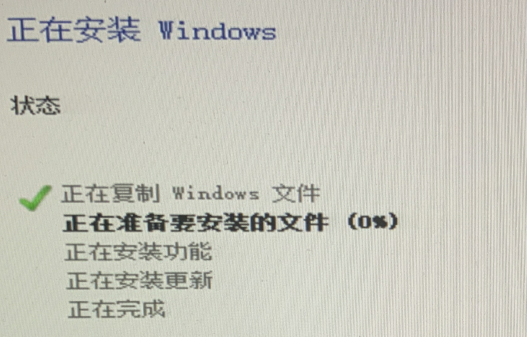
\includegraphics[scale=0.3]{18}
\end{figure}

18.安装完成后,会自动重启。在开机界面按F11进入启动设备选项,进入Windows。
\begin{figure}[htbp]
	\centering
	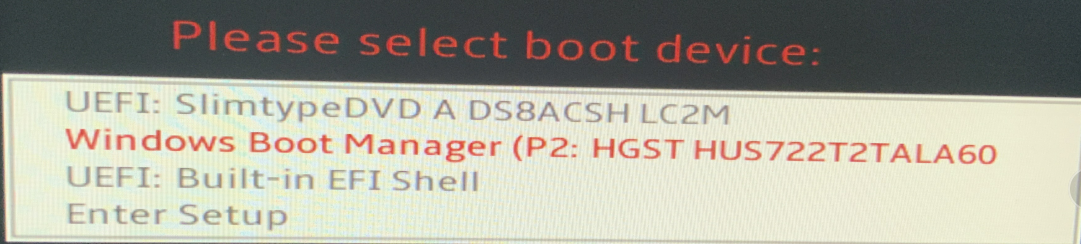
\includegraphics[scale=0.3]{19}
\end{figure}

19.进入之后设置区域。
\begin{figure}[htbp]
	\centering
	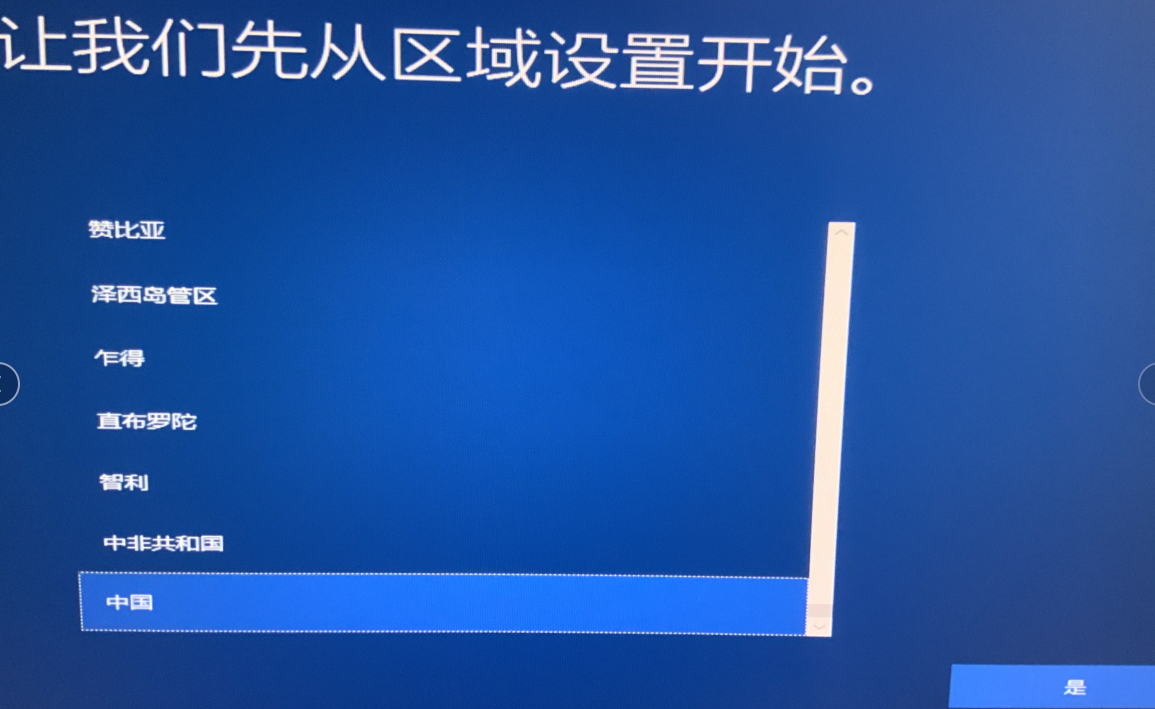
\includegraphics[scale=0.24]{20}
\end{figure}

20.设置键盘布局。
\begin{figure}[H]
	\centering
	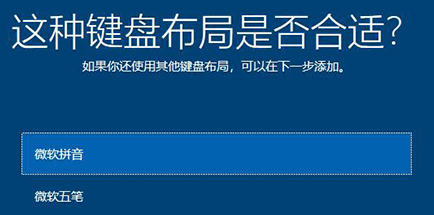
\includegraphics[scale=0.45]{a}
\end{figure}

20.设置个人还是组织。
\begin{figure}[htbp]
	\centering
	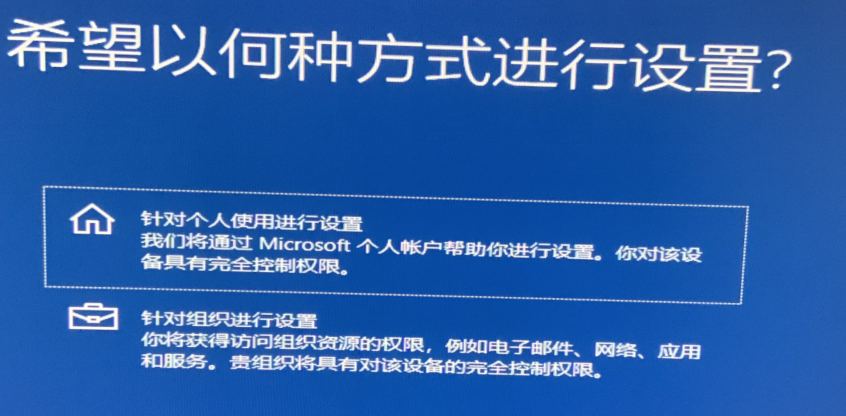
\includegraphics[scale=0.24]{21}
\end{figure}

21.设置用户
\begin{figure}[H]
	\centering
	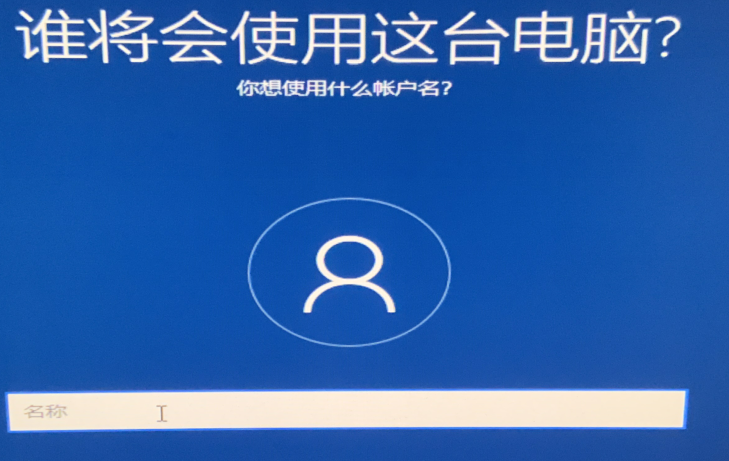
\includegraphics[scale=0.24]{b}
\end{figure}

22.设置密码
\begin{figure}[htbp]
	\centering
	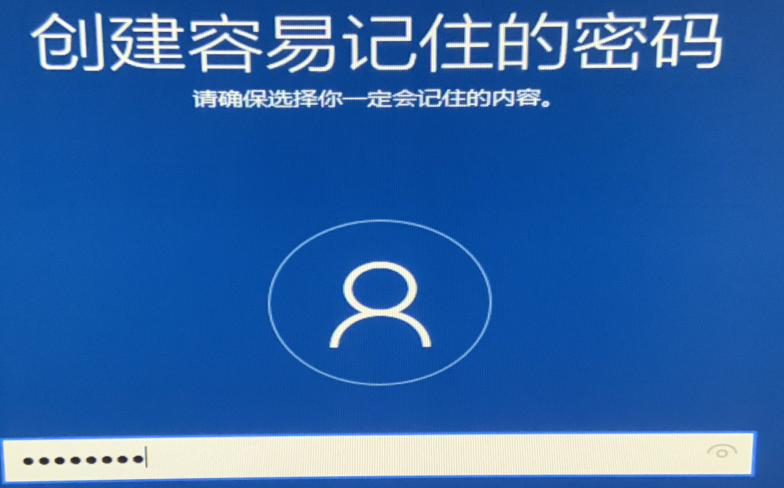
\includegraphics[scale=0.24]{c}
\end{figure}

23.为此账户创建安全问题
\begin{figure}[H]
	\centering
	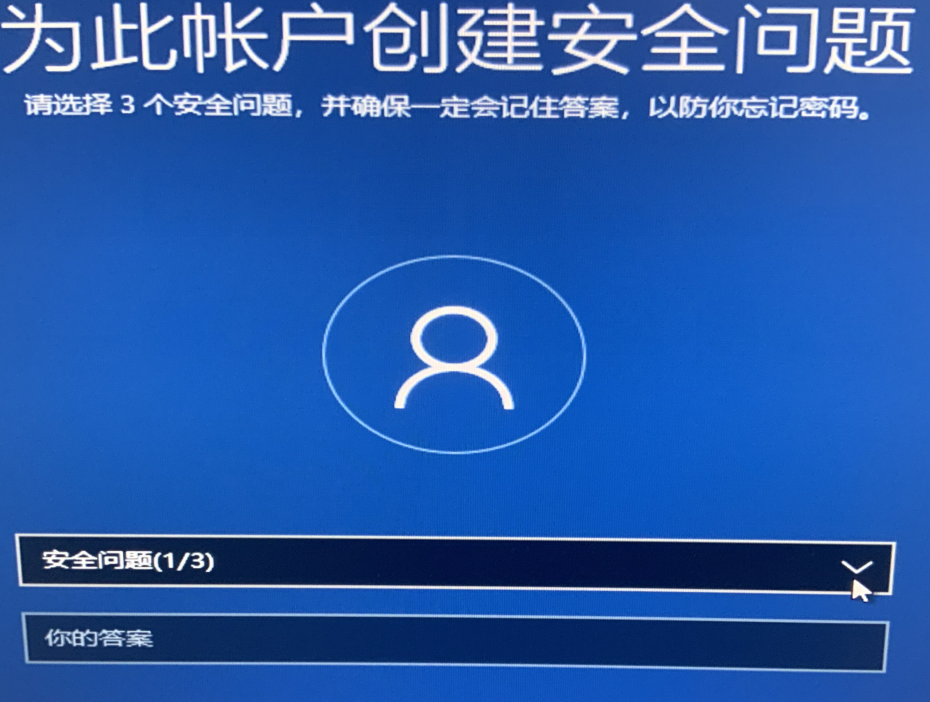
\includegraphics[scale=0.2]{22}
\end{figure}

24.个人助理设置
\begin{figure}[H]
	\centering
	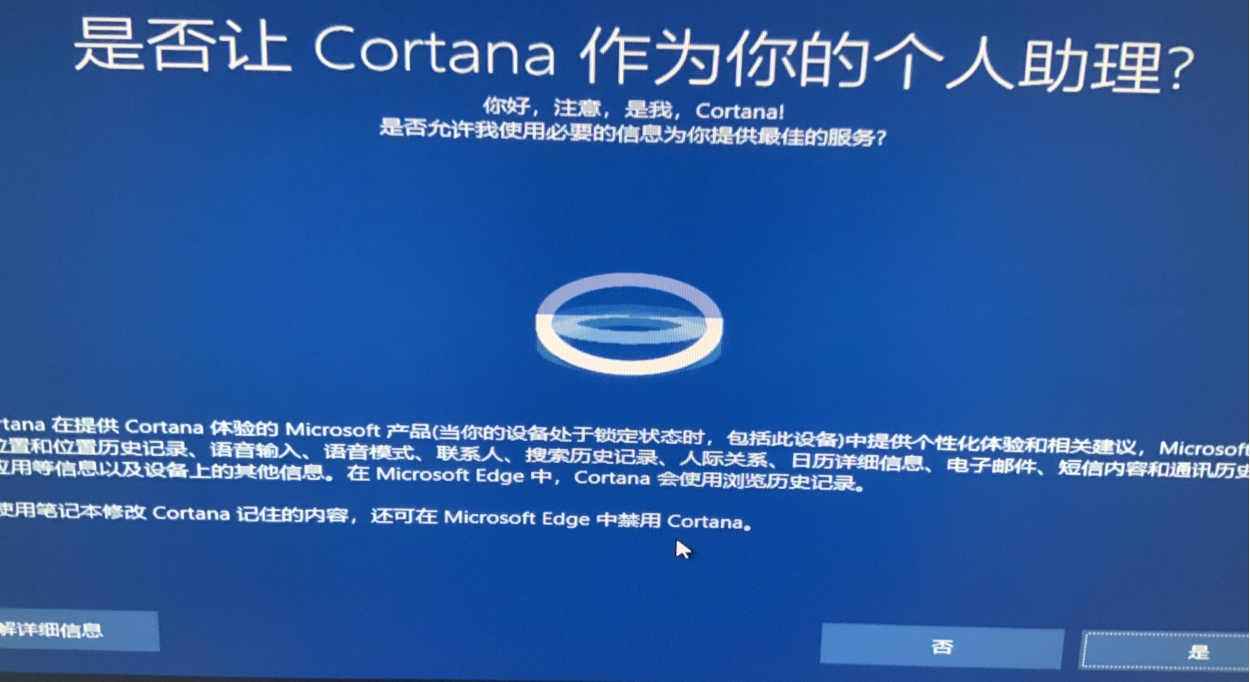
\includegraphics[scale=0.24]{23}
\end{figure}

25.隐私设置
\begin{figure}[htbp]
	\centering
	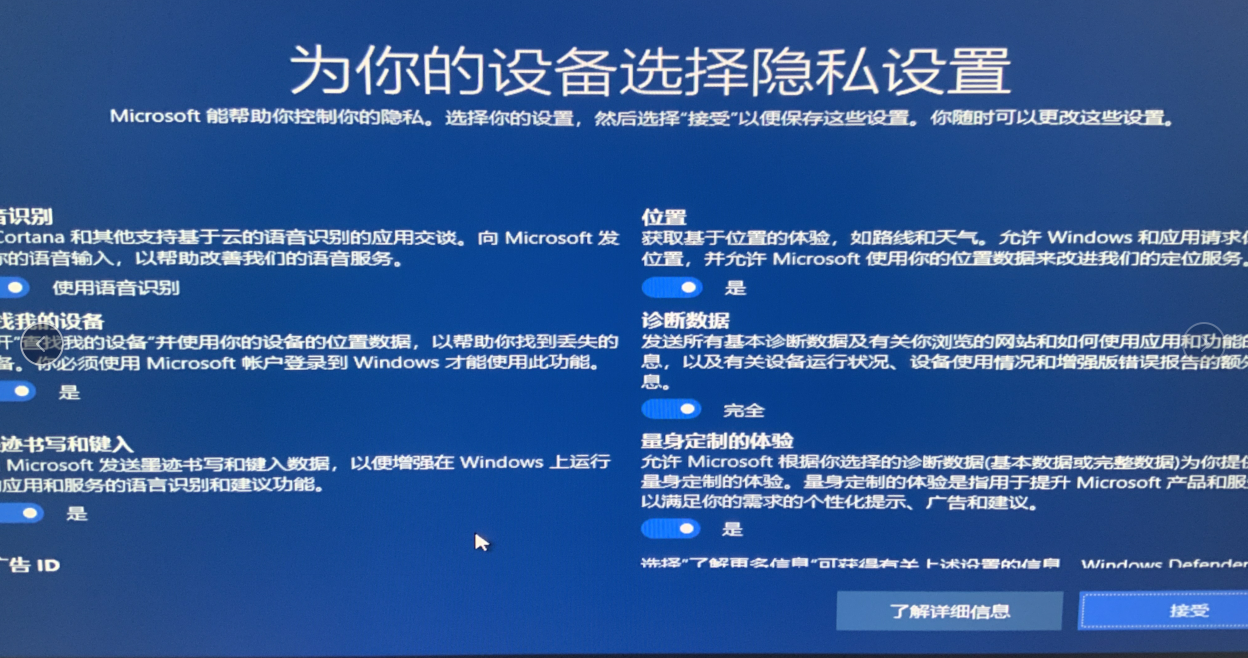
\includegraphics[scale=0.24]{24}
\end{figure}

26.之后进入windows界面,参考下面的安装步骤。
\subsection{安装恢复软件}

本系统为用户提供Windows系统下一键式自动安装功能.

操作流程:进入Windows系统之后启动网络管理安装程序,安装完成。

操作步骤:

Step1:双击本系统安装程序,选择语言:
\begin{figure}[H]
	\centering
	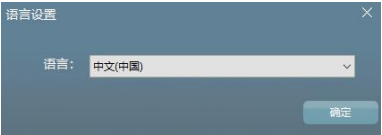
\includegraphics[scale=0.3]{语言设置}
\end{figure}

Step2:点击“安装”按钮,完成安装。
\begin{figure}[H]
	\centering
	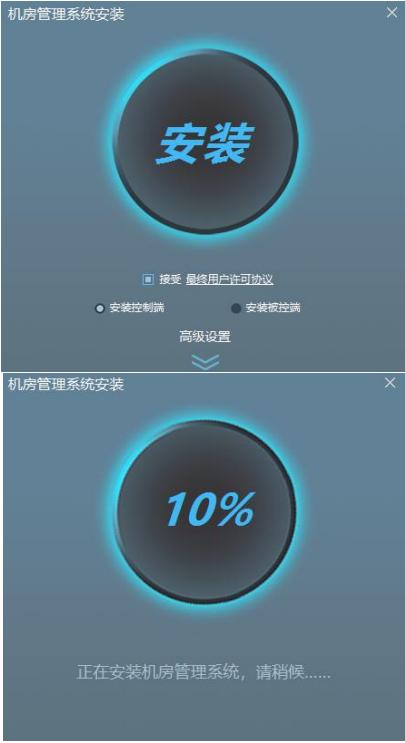
\includegraphics[scale=0.3]{系统安装1}
\end{figure}

Step3:出现以下界面即为安装完成
\begin{figure}[htbp]
	\centering
	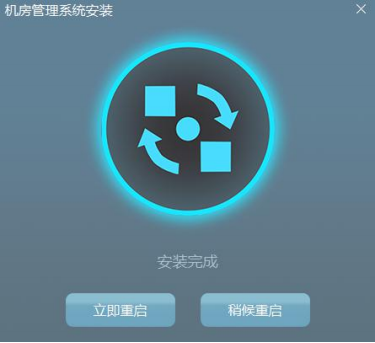
\includegraphics[scale=0.3]{系统安装2}
\end{figure}

Step4:拔掉外置光驱,重启电脑

如果开机有问题,请进入Bios系统,设置第一启动项为硬盘启动。
\subsection{恢复软件中的设置}
开机完出现
\begin{figure}[htbp]
	\centering
	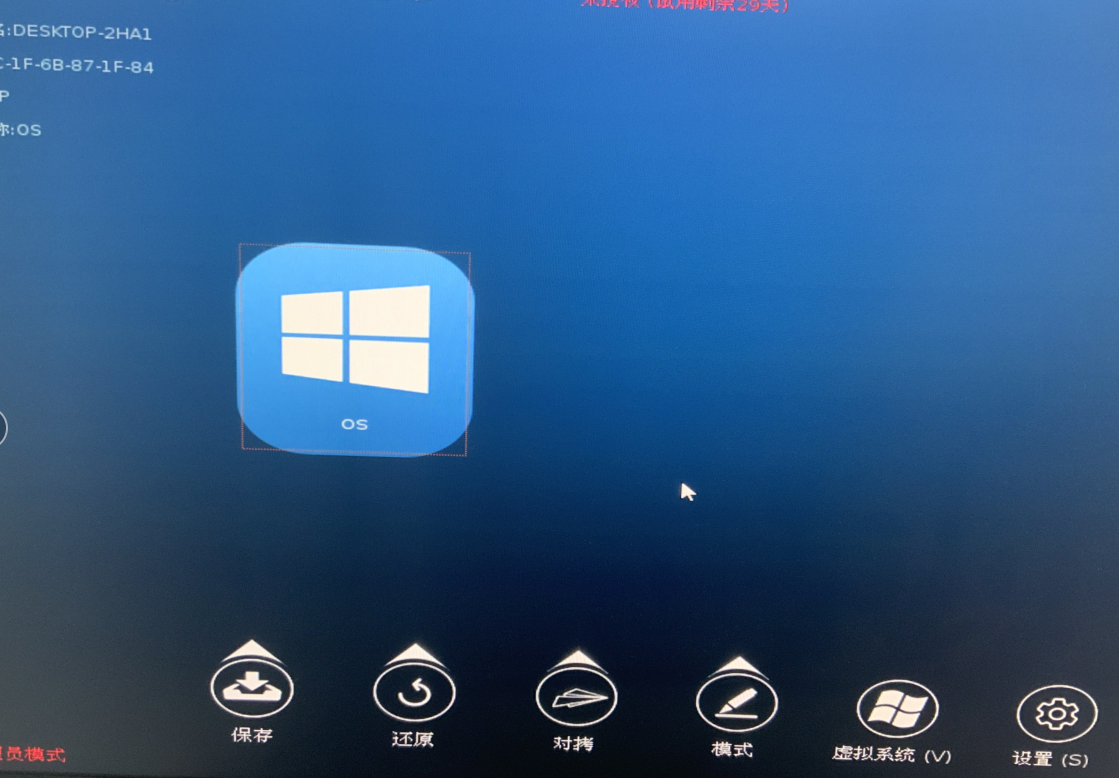
\includegraphics[scale=0.3]{25}
\end{figure}

1.选择设置,密码默认为admin。选择分区管理。
\begin{figure}[H]
	\centering
	
\includegraphics[scale=0.3]{26}
\end{figure}

2.新建分区,具体参数如下。点击应用,确定,返回。
\begin{figure}[H]
	\centering
	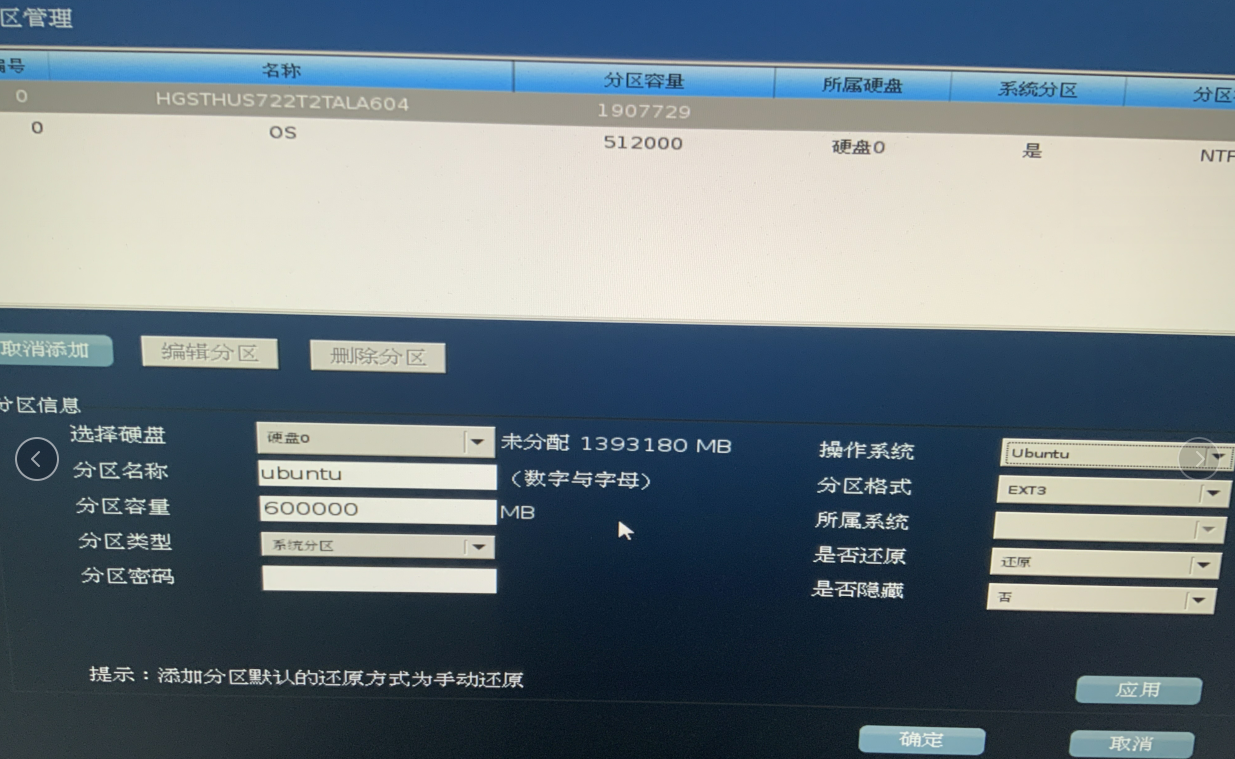
\includegraphics[scale=0.3]{27}
\end{figure}

3.之后能看到以下界面
\begin{figure}[H]
	\centering
	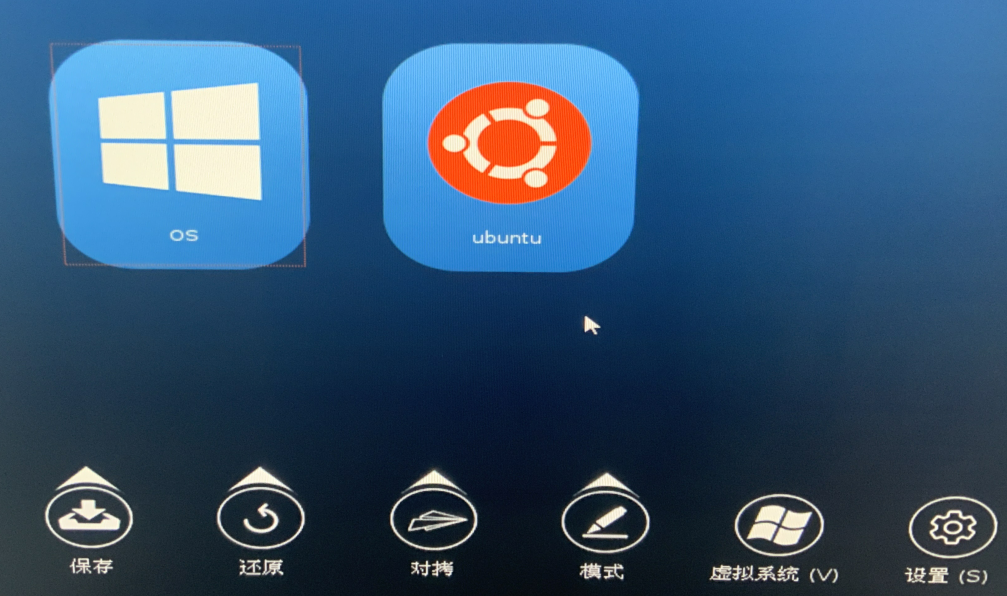
\includegraphics[scale=0.3]{28}
\end{figure}
\subsection{Ubuntu安装}
1.换ubuntu的安装光盘,之后点击ubuntu,进入。按F11进入启动项选择界面,选择外置USB CD启动

2.中途会出现选安装类型,根据需要自己选择。之后等待。

3.进入之后,双击桌面上的安装程序。
\begin{figure}[H]
	\centering
	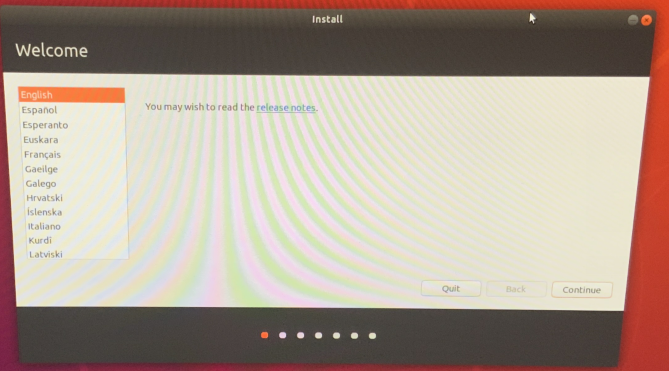
\includegraphics[scale=0.3]{29}
\end{figure}

4.设置语言为中文
\begin{figure}[H]
	\centering
	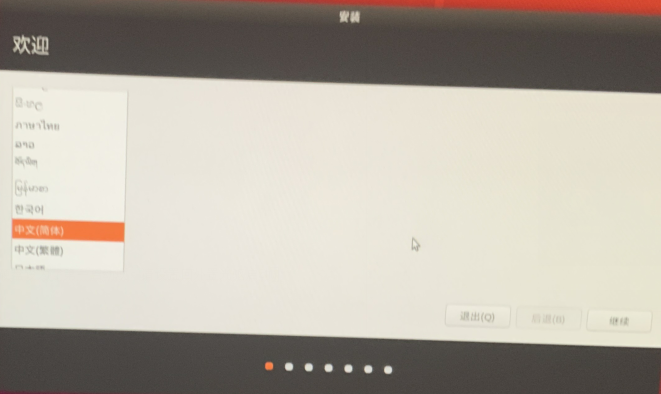
\includegraphics[scale=0.3]{30}
\end{figure}

5.设置键盘布局
\begin{figure}[H]
	\centering
	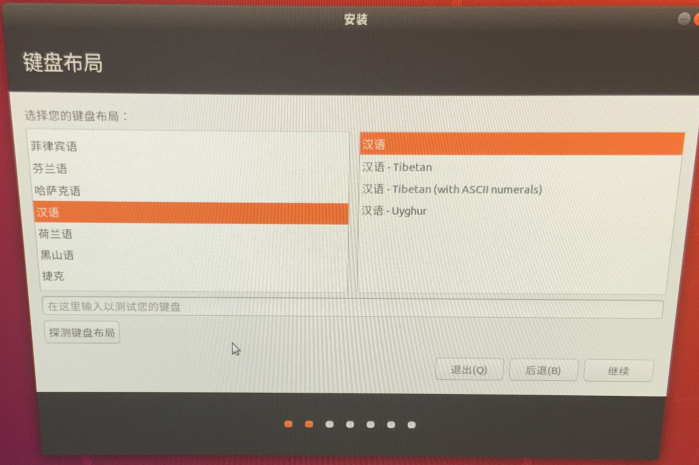
\includegraphics[scale=0.3]{31}
\end{figure}

6.设置更新和其他软件
\begin{figure}[H]
	\centering
	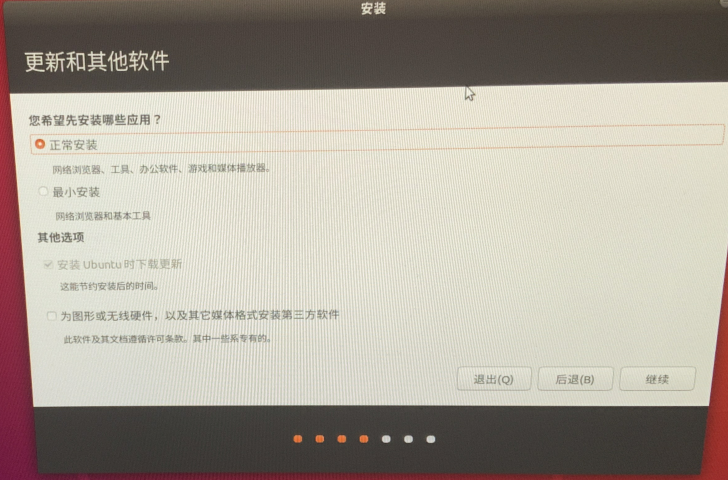
\includegraphics[scale=0.3]{32}
\end{figure}
请注意不要选择"为图形或无线硬件,以及MP3和其他媒体安装第三方软件。

7.安装类型选择
\begin{figure}[H]
	\centering
	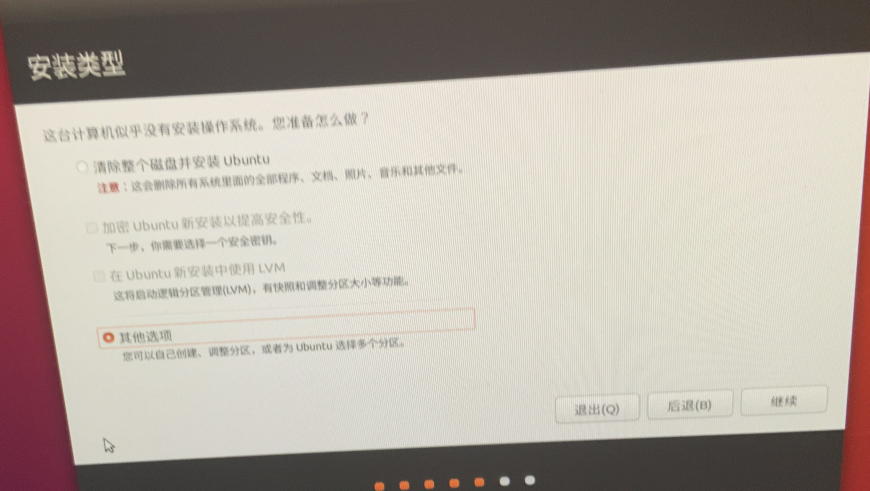
\includegraphics[scale=0.3]{33}
\end{figure}

8.选择之前所分出来的Ubuntu的区盘,点击更改。
\begin{figure}[H]
	\centering
	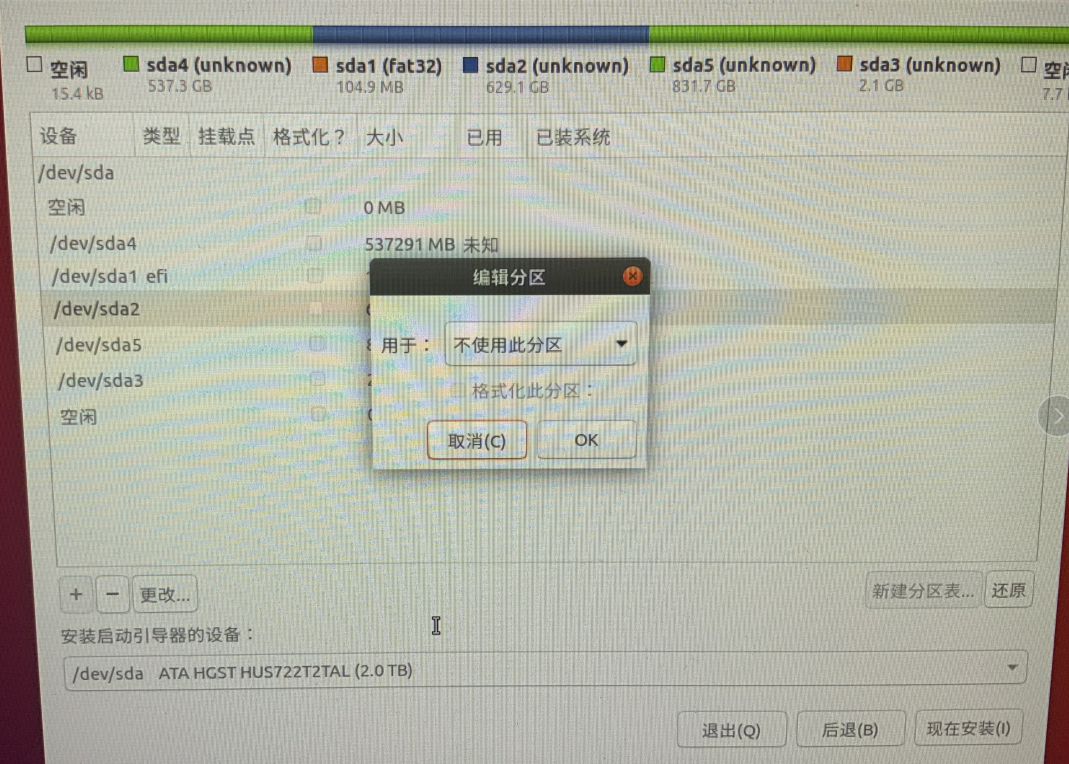
\includegraphics[scale=0.3]{34}
\end{figure}

9.将其修改为如下图所示。
\begin{figure}[H]
	\centering
	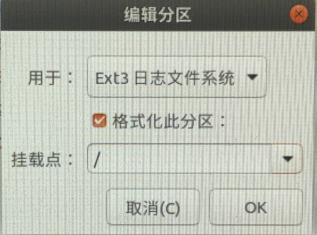
\includegraphics[scale=0.3]{35}
\end{figure}

10.选择区盘进行安装
\begin{figure}[H]
	\centering
	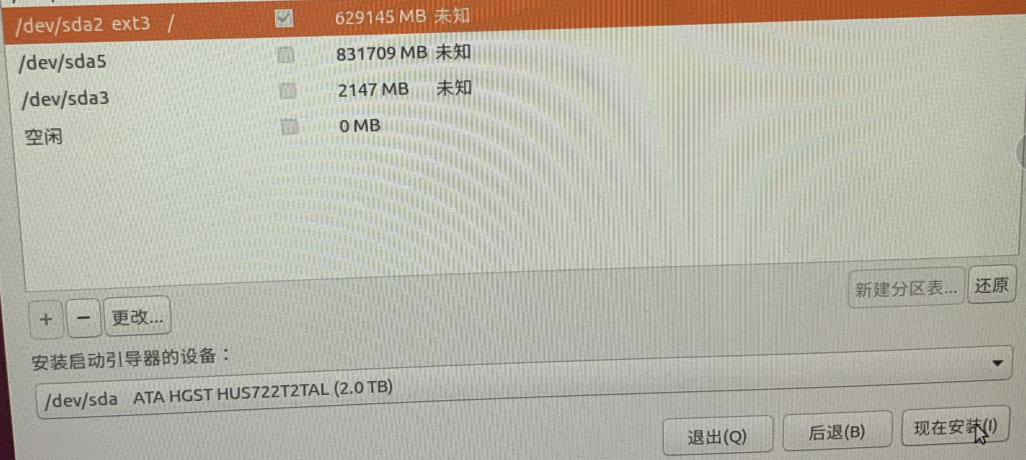
\includegraphics[scale=0.3]{36}
\end{figure}

11.等待,选择上海,继续
\begin{figure}[H]
	\centering
	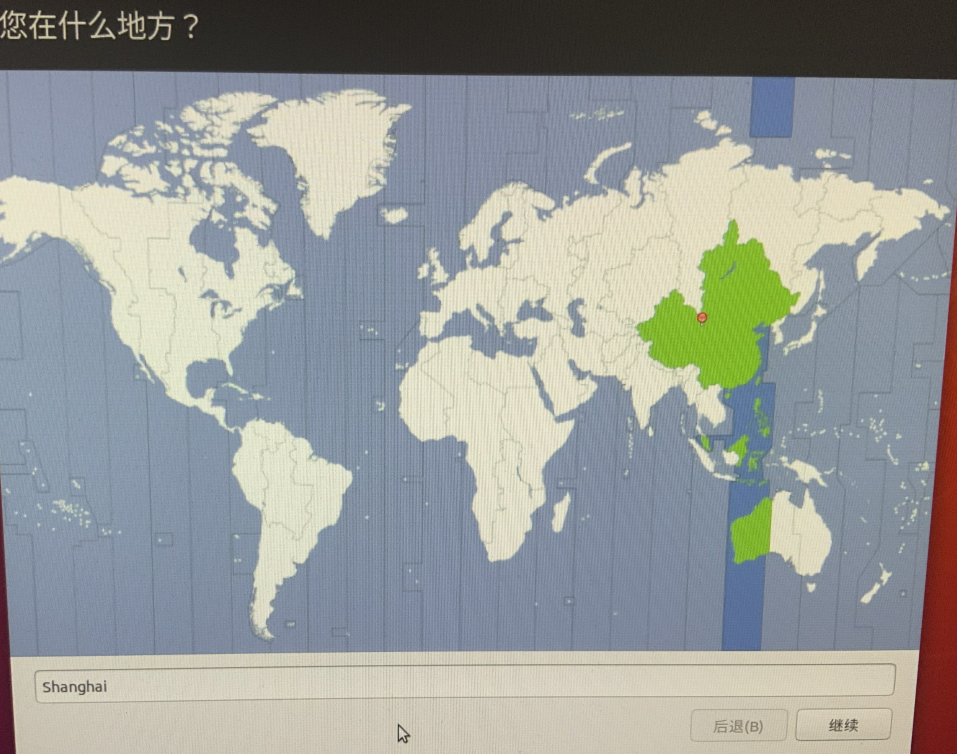
\includegraphics[scale=0.3]{37}
\end{figure}

12.设置用户名和密码
\begin{figure}[H]
	\centering
	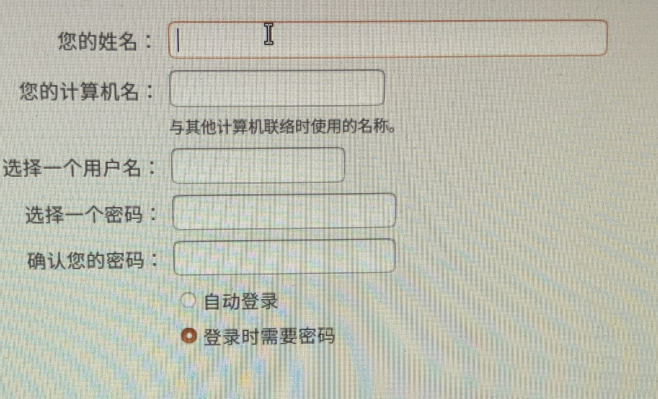
\includegraphics[scale=0.3]{38}
\end{figure}

13.等待安装重启,拔出外置光驱。之后进入ubuntu系统,安装Linux驱动。
\subsection{Linux驱动安装}
Linux系统驱动安装

操作流程:进入Linux系统,执行安装程序,安装完成

操作步骤:

1:将驱动文档(压缩包)拷贝到Linux系统桌面目录下,单击右键启动Terminal终端
\begin{figure}[H]
	\centering
	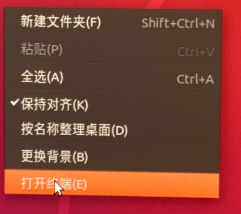
\includegraphics[scale=0.3]{39}
\end{figure}

2:执行sudo su代码,回车
\begin{figure}[H]
	\centering
	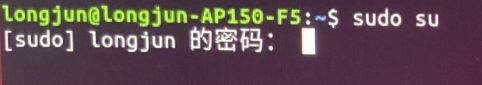
\includegraphics[scale=0.3]{40}
\end{figure}

3.输入密码(注意这里输入的密码没有显示,隐藏了)
\begin{figure}[H]
	\centering
	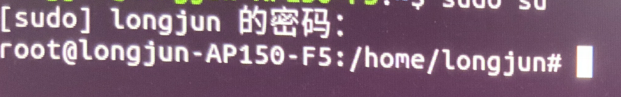
\includegraphics[scale=0.3]{41}
\end{figure}

4.执行cd 桌面命令,进入桌面。
\begin{figure}[H]
	\centering
	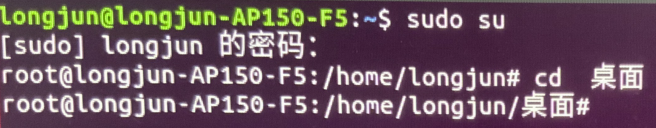
\includegraphics[scale=0.3]{42}
\end{figure}

5.执行tar -zxvf linuxdrive.tgz命令,解压压缩包。
\begin{figure}[H]
	\centering
	\includegraphics[scale=0.3]{43}
\end{figure}

6.执行cd linuxtool20210331ib/命令,进入压缩包
\begin{figure}[H]
	\centering
	\includegraphics[scale=0.3]{44}
\end{figure}

7.执行./main命令
\begin{figure}[H]
	\centering
	\includegraphics[scale=0.3]{45}
\end{figure}

8.等待安装,出现done,即为安装完成。关闭终端。重启电脑,按delete,进bios,第一启动项设为硬盘启动
\begin{figure}[H]
	\centering
	\includegraphics[scale=0.3]{46}
\end{figure}

\section{Ubuntu系统软件安装}
\subsection{NVIDIA驱动安装}
\subsubsection{禁用nouveau}
1.验证nouveau开启了(命令之后会有输出)

lsmod | grep nouveau

2.打开编辑配置文件

sudo gedit /etc/modprobe.d/blacklist.conf

3.在出现的文档最后一行添加以下命令,保存。禁用第三方驱动

blacklist nouveau

4.使命令生效

sudo update-initramfs -u

5.重启

sudo reboot

6.验证nouveau禁用(命令后没有输出)

lsmod | grep nouveau

\begin{figure}[H]
	\centering
	\includegraphics[scale=0.3]{50}
\end{figure}
\subsubsection{安装驱动}  
1.查看显卡

ubuntu-drivers devices

2.去NVDIA driver search page(\texttt{https://www.nvidia.com/Download/index.aspx})查看支持显卡的驱动的最新版本的版本号

3.安装相关包

sudo apt update

sudo apt install build-essential

gcc $--$version

4.安装下载好的驱动(...指驱动的名字省略)

sudo bash NVIDIA-Linux....

5.重启电脑

sudo reboot

6.查看显卡信息

nvidia-smi

\subsection{安装cuda}
1.在下列的网站中下载符合要求的cuda

\texttt{https://developer.nvidia.com/cuda-toolkit-archive}

2.安装cuda,执行以下命令(...指cuda的名字省略)。选择安装部件时不选显卡驱动。

sudo sh cuda... 

3.配置cuda环境

sudo vim ~/.bashrc

在该文件中加入以下命令

export CUDA\_HOME=/usr/local/cuda-11.1

export LD\_LIBRARY\_PATH=/usr/local/cuda-11.1/lib64:\$LD\_LIBRARY\_PATH

export PATH=/usr/local/cuda-11.1/bin:\$PATH

4.更新cuda环境

source $\sim$/.bashrc

5.验证cuda环境
nvcc $--$version

\begin{figure}[H]
	\centering
	\includegraphics[scale=0.4]{51}
\end{figure}

\subsection{安装cudnn}
1.在下列的网站中下载符合要求的cudnn

\texttt{https://developer.nvidia.com/rdp/form/cudnn-download-survey}

选择cuda版本对应的cudnn点开后选择 cudnn library for linux,点击下载。(最好选择 cudnn library for linux 这个文件格式安装比较方便)

2.复制cudnn头文件

sudo cp cuda/include/* /usr/local/cuda-11.1/include/

3.复制cudnn的库

sudo cp cuda/lib64/libcudnn* /usr/local/cuda-11.1/lib64/

4.添加可执行权限

sudo chmod +x /usr/local/cuda-11.1/include/cudnn.h

sudo chmod +x /usr/local/cuda-11.1/lib64/libcudnn*

5.查看cudnn的版本号

cat /usr/local/cuda/include/cudnn.h | grep CUDNN\_MAJOR -A 2

\begin{figure}[H]
	\centering
	\includegraphics[scale=0.4]{52}
\end{figure}
\section{配置环境}
\subsection{安装Anaconda}
1.更新本地文件

sudo apt-get update

2.在下面的连接下载最近版本的Anoconda

https://www.anaconda.com/

3.在/usr/local中进入终端,在命令行中进入root权限.

mkdir Anaconda3

4.运行下载下来的Anaconda安装包,进行安装

sudo bash Anaconda3-2021.05-Linux-x86\_64.sh -p /usr/local/Anaconda3 -u 

5.加入Anaconda路径

sudo gedit $\sim$/.bashrc

在文档最后加入
export PATH= /usr/local/anaconda3/bin:\$PATH

更新路径

source $\sim$/.bashrc

关闭终端,重开终端验证conda是否装好

conda info

也能验证python是否安装好:

python

\begin{figure}[H]
	\centering
	\includegraphics[scale=0.5]{53}
\end{figure}

\subsection{Anaconda配置虚拟环境}

创建环境命令:
sudo conda creat $--$name test\_environment python=3.8 

查看现有的虚拟环境:
conda info $--$envs

激活现有的环境:
conda activate test\_environment

删除现有的环境:
conda remove $--$name text\_environment $--$all 

给环境安装包

\begin{figure}[H]
	\centering
	\includegraphics[scale=0.05]{54}
\end{figure}
\subsubsection{无法创建环境}
解决sudo conda无法创建环境,运行以下命令

vim $\sim$/.bashrc

在文件最后加入以下命令

alias sudo="sudo env PATH=\$PATH"

更新设置

source $\sim$/.bashrc

重新打开终端进行创建环境。

\begin{figure}[H]
	\centering
	\includegraphics[scale=0.5]{61}
\end{figure}
\subsection{Linux系统备份}
1.上述操作重启电脑后,确保是管理员模式,进入管理界面。点击设置,分区管理。在如图配置再添加一个分区
\begin{figure}[H]
	\centering
	\includegraphics[scale=0.3]{47}
\end{figure}

2.模式切换为还原模式,点击保存中的linux分区。
\begin{figure}[H]
	\centering
	\includegraphics[scale=0.3]{48}
\end{figure}

3.勾选安装了Ubuntu的分区。
\begin{figure}[H]
	\centering
	\includegraphics[scale=0.3]{49}
\end{figure}

4.等待备份结束。

\subsection{Windows系统备份}
1.模式切换为还原模式,点击保存中的Windows分区。

2.勾选安装了Windows的分区。

3.等待备份结束。

\section{系统进行连接}
\subsection{发送端设备准备}
1.进入本系统底层启动界面,按“Ctrl+C”键->输入管理员密码->进入对拷主界面

2.点击批量部署,选择UEFI,等待接收端登陆。
\begin{figure}[H]
	\centering
	\includegraphics[scale=0.4]{59}
\end{figure}

\begin{figure}[H]
	\centering
	\includegraphics[scale=0.5]{60}
\end{figure}
\subsection{接收端设备准备}
开机进bios管理设置,在Advanced中找到PCIe/PCI...进入。
\begin{figure}[H]
	\centering
	\includegraphics[scale=0.05]{57}
\end{figure}

将配置调成以下配置
\begin{figure}[H]
	\centering
	\includegraphics[scale=0.05]{55}
\end{figure}
\begin{figure}[H]
	\centering
	\includegraphics[scale=0.05]{56}
\end{figure}

之后保存重启。按F11进入开启启动项选项界面,选择PXE IP4...
\begin{figure}[H]
	\centering
	\includegraphics[scale=0.05]{58}
\end{figure}

待发送端进入发送界面后,再按回车进行接收端登陆。

\end{document}